\titre{Clique :} Une clique de taille $n$ est un sous graphe complet de taille $n$ ($K_n$). Une anticlique de taille $n$ est un sous graphe vide de taille $n$ ($\bar{K_n}$). \\

\titre{Théorème de Ramsey :} Pour tout entier $k \geq 1, \exists R_k \in \N$ tel que tout graphe possédant au moins $R_k$ sommets contient au moins une clique ($K_k$) ou une anticlique ($\bar{K_k}$) de taille $k$. \\

\titre{Exemple :}\\
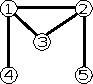
\includegraphics[width=60px]{Images/01_exRamsey.pdf} \\
$\begin{array}{|c|c|}
	 k & R_k \\ \hline
	 1 & 1 \\ \hline
	 2 & 2 \\ \hline
	 3 & 6 \\ \hline
	 4 & 18 \\ \hline
	 5 & \in [43;49] \\ \hline
	 6 & \in [102;165] \\ \hline
	 17 & \in [8917;601080389] \\ \hline
\end{array}$
\\

\titre{Essai d'algorithme naïf :} On cherche tous les graphes de chaque taille et on cherche un contre exemple. \\
Pour une taille $N$ donné il existe $2^{\frac{N(N-1)}{2}}$ graphes possibles. \\
Pour chaque graphe possible on va tester tous les sous graphes de taille $k$ donc $\frac{N!}{k!(N-k)!}$. \\
Puis pour chacun il faut vérifier que c'est une clique ou une anticlique donc $\frac{k(k-1)}{2}$. \\
Et il faut itérer sur $N$ pour chercher un contre exemple. \\
Pour $N = 8$ et $k = 4$ le programme ne terminera pas de notre vivant. \\

\titre{Représentation d'une instance :} Graphe dont les sommets sont des entiers. \\
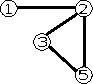
\includegraphics[width=50px]{Images/02_exEncodage.pdf}\\
Symboles = $\{ (,),0,1,2,3,4,5,6,7,8,9,- \}$. \\
Schéma = $(1-2-3-5)(1-2-3-5-2-3-2-5)$ représente le graphe ci-dessus avec une taille 26.\\

\titre{Cycle Eulérien :} Passe une et une seule fois par chacune des arêtes. \\

\titre{Théorème :} Un graphe $G$ est eulérien \ssi il est connexe et tous ses sommets sont de degré pair. \\

\titre{Preuve :}
\begin{itemize}
	\item $\impl$ Si $G$ a un sommet de degré impaire, il ne peut pas être eulérien car chaque passage dans un sommet diminue son degré de 2.
	\item $\implinv$ Si $G$ a tous ses sommets de degré pair, dès qu'on arrive sur un sommet, on peut sortir, donc on revient forcément au début. Pour chaque sommet dont tous les voisins n'ont pas été visités, on choisit une arête sortante non visitée, par le même raisonnement on revient à ce sommet au bout d'un moment. On intègre le cycle obtenu au cycle de départ et on recommence, jusqu'à ce que toutes les arêtes aient été visitées.
\end{itemize}

\titre{Cycle Hamiltonnien :} Passe une et une seule fois par chacun des sommets. \\
